%%%%%%%%%%%%%%%%%%%%%%%%%%%%%%%%%%%%%%%%%%%%%%%%%%%%%%%%%%%%%%%%%%%%%%%
%%%                           System Description
%%%%%%%%%%%%%%%%%%%%%%%%%%%%%%%%%%%%%%%%%%%%%%%%%%%%%%%%%%%%%%%%%%%%%%





\chapter{System Description}

In this chapter, we will talk about designing the game, the story, mechanics, and tools used, and results from some of the initial studies that we conducted, as we iterated on the game design.

\section{Game Description}
The game is developed on React\footnote{https://reactjs.org/} with Chakra UI\footnote{https://chakra-ui.com}. We use Supabase\footnote{https://supabase.com/} to keep logs of user interaction with the game. Figure \ref{fig:screenshot} shows the initial state of the game.

\begin{figure}[h]
    \centering
    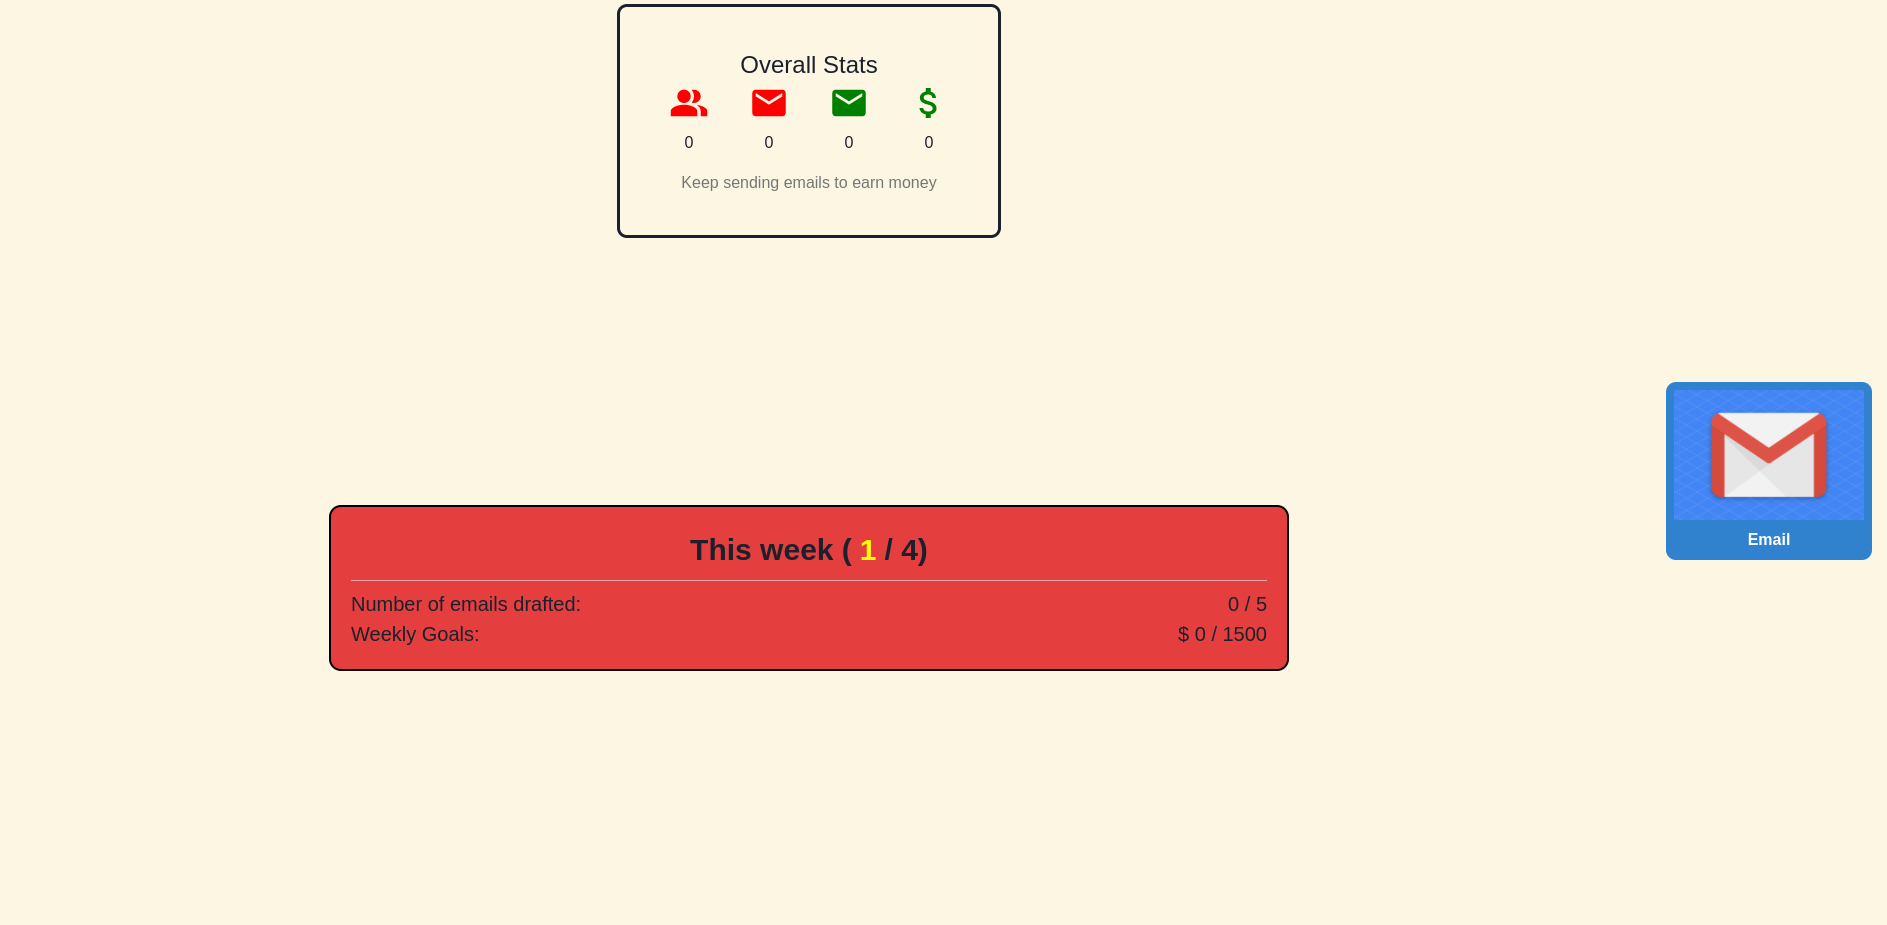
\includegraphics[width=1 \textwidth]{figures/section2/game.png}
    \caption{Screenshot of initial state of the game}
    \label{fig:screenshot}
\end{figure}

\subsection{Game Story}
The game's main character has taken a large loan from a loan shark. The goal of the game is to pay off the loan in time. However, as the loan is substantial, he cannot earn enough money through hard work and uses phishing tricks to scam people. The main character hires a helper to create phishing emails based on his input and impersonates PayPal to trick victims and earn money. The player has four weeks to pay off the loan with weekly payment. Each week unlocks new skills to help the player create more effective emails.

\section{Mechanics}
One of our main objectives while developing the game was to streamline the player experience. We divided the game into four weeks (parts) to achieve this goal. Each week's progression will lock/unlock specific skills users' can use to create email. We will talk more about certain week progression in later sections. Players can use the unlocked skills to generate emails. Each email efficiency will be based on the option chosen by the user.

\subsection{Components}
Before we deep dive into the flow of the game, let us talk about each individual component.

\subsubsection{Atttacker}
The attacker module takes care of training the helper. There are six different skills that the player can train the helper on, namely spelling, grammar, styling, links, spoofing, and research. We divide these skills as language skills (spelling and grammar) and technical skills (styling, links, spoofing, research). Language skills are passive skills in the game, whereas technical skills, except for styling, are active skills.

Training on passive skills will improve the quality of the email generated by the system without any additional input from the user. In contrast, active skills will give the user more options while generating the email. For example, after you train you helper on spellings, the attacker will stop making spelling errors without any additional input from the user. However, training the helper on links will allow the user to choose how to hide the links while creating the email. Table \ref{table:attacker} lists the skills and their effect in the game in brief. We will talk about the different properties activated by each skill while talking about email generation.

\begin{table}[h]
    \begin{tabular}{  p{0.1\textwidth}  p{0.17\textwidth}  p{0.45\textwidth}  }
        \hline
        \textbf{Skills} & \textbf{Active/Passive} & \textbf{Effect}                                                   \\
        \hline
        Spelling        & Passive                 & Creates emails without spelling errors                            \\
        Grammar         & Passive                 & Create emails without grammar errors                              \\
        Styling         & Passive                 & Create stylized emails with better header, footer, and images     \\
        Links           & Active                  & Unlocks different techniques to hide the link while sending email \\
        Research        & Active                  & Gives the user option to generated targeted emails                \\
        Spoofing        & Active                  & Gives the user ability to spoof the email                         \\
        \hline
    \end{tabular}
    \caption{Different skills and their effect in the game}
    \label{table:attacker}
\end{table}

We chose the skills in the game to replicate existing training modules objectives. We could not itemize some general properties of phishing emails such as sense of urgency, generic greetings, too good to be true emails, etc. However, we have integrated these common traits in the generated emails.

\subsubsection{Marketplace}
- domains, buying domains
- distance formula
- trancos' list

\subsubsection{Email Generation}
- how emails are generated
- efficiency


\subsection{Previous Iteration}
- talk about time constraints and why we removed them

\subsection{Weekly Goals}


